\section{RAID one}

RAID one is a type of data storage configuration where data is duplicated (mirrored) to a second disk. 
This provides high reliability, as when a disk fails, the second copy can be used. 
Reads of data can be retrieved from the disk with shorter queueing, seek, and latency delays.
However, writes are slower than standard disks due to the duplication, and the cost of using 50\% of the capacity is higher.

In principle, a RAID 1 can mirror the content over more than one disk. 
This provides resiliency to errors even if more than one disk breaks.
Additionally, with a voting mechanism, it allows for the identification of errors not reported by the disk controller. 
However, in practice, this is never used because the overhead and costs are too high.

\subsection{Mirroring}
The key idea for mirroring is to make two copies of all data. 
This provides data redundancy, which means that if one copy of the data is lost or corrupted, the other copy can be used to recover the data. 
This provides a level of fault tolerance and data protection that is not present in RAID 0, which offers high performance but no error recovery.
By making two copies of all data, mirroring provides both high performance and data protection.

If multiple disks are available, they can be coupled in an even number to achieve a total capacity that is halved. 
Each disk can have a mirror, and RAID levels can be combined to achieve the desired performance and redundancy. 
The two possible combinations are RAID $01$ and RAID $10$.

\subsection{Multiple levels RAID}
RAID levels can be combined by considering the number of groups of disks and applying RAID $x$ to each group of $n$ disks. 
Then, RAID $y$ can be applied to the $m$ groups of $n$ disks, resulting in a total of $n \times m$ disks.
\begin{figure}[H]
    \centering
    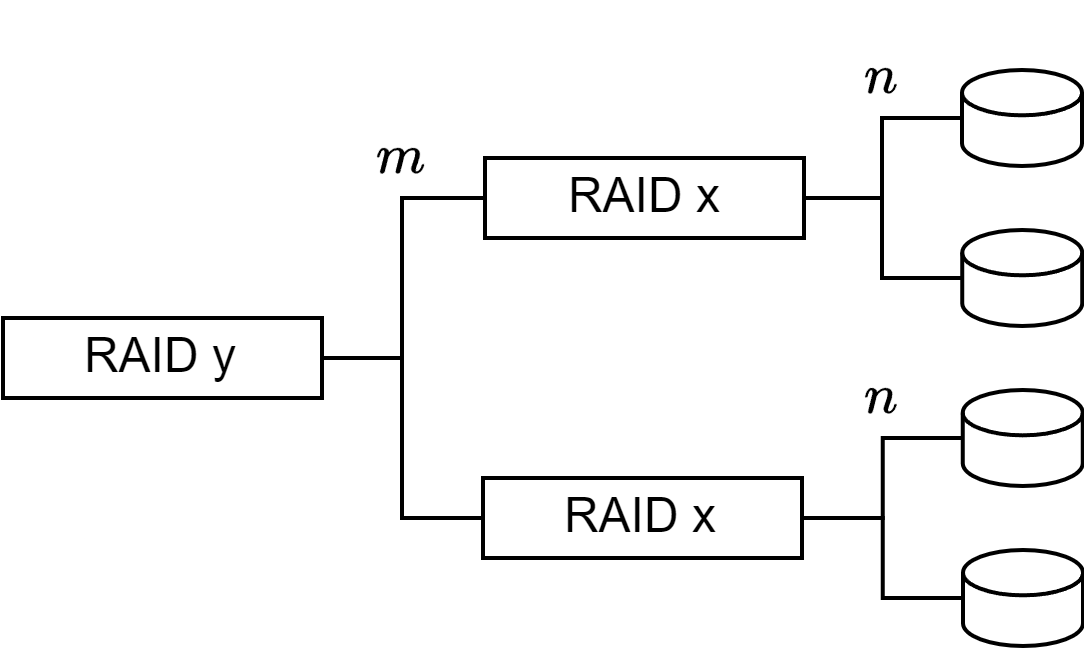
\includegraphics[width=0.5\linewidth]{images/level.png}
    \caption{RAID levels}
\end{figure}

\paragraph*{RAID 01}
RAID level 0 + 1 is a type of RAID (Redundant Array of Independent Disks) configuration where data is first striped across multiple drives using RAID 0, and then mirrored using RAID 1. 
This provides both high performance and data redundancy. 
In the event of a failure of one of the drives in the RAID 0 stripe, the data is still available on the other drives, and the RAID 1 mirror provides an additional copy of the data for protection. 
The minimum number of drives required for this configuration is four.

\paragraph*{RAID 10}
RAID 10 is a type of RAID (Redundant Array of Independent Disks) level that combines the mirroring of RAID 1 with the striping of RAID 0. 
In RAID 10, data is first mirrored across two or more drives (RAID 1), and then the mirrored data is striped across the remaining drives (RAID 0). 
This provides both data redundancy and improved performance for read and write operations.
RAID 10 is commonly used in databases with very high workloads, particularly those that require fast writes.
A minimum of four drives are required to implement RAID 10.

\subsection{Comparison}
RAID 0, 1, 0+1, and 1+0 organizations differ in the order of block allocation.
Both RAID 10 and RAID 01 have the same performance. 
The storage capacity of RAID 10 and RAID 01 is the same.
The main difference between these RAID organizations is their fault tolerance levels:
\begin{itemize}
    \item RAID 0+1 has less fault tolerance on most RAID controller implementations.
    \item RAID 1+0 has a larger fault tolerance level.
\end{itemize}

\subsection{Summary}
The following is a summary of the features of RAID 1:
\begin{itemize}
    \item The system has a capacity of $\frac{N}{2}$, meaning it can store half of the total data.
    \item The system has a reliability of $1$, meaning that if one drive fails, the system can still function without data loss.
        However, if multiple drives fail, the system may not be able to recover all of the data. 
        In the best-case scenario, $\frac{N}{2}$ drives can fail without data loss.
    \item The system supports sequential read and write operations of $\frac{N}{2}\times S$, which means that it can read and write half of the data in the system at a time.
        This results in a throughput of $\frac{N}{2}\times S$.
    \item The system also supports random read and write operations of $\frac{N}{2}\times R$, which means that it can read and write half of the read blocks in the system at a time. 
        However, since only half of the read blocks are actually being read, this results in half of the read throughput.
\end{itemize}
In the best scenario, it is possible to have $\frac{N}{2} \times R$ random writes, where $N$ is the number of disks and $R$ is the number of random writes per disk. 
This is because we have two copies of all data, so the throughput is halved. 
On the other hand, reads can parallelize across all disks, so it is possible to have $N \times R$ random reads in the best scenario.